\documentclass{article}

\usepackage{graphicx}
\usepackage{tikz}
\usepackage{tikzsymbols}
\usetikzlibrary{calc,patterns,shapes.geometric}
\pagestyle{empty}
\usepackage[margin=0pt]{geometry}
\geometry{papersize={14in,12in}}

\def\centerarc[#1](#2)(#3:#4:#5){\draw[#1] ($(#2)+({#5*cos(#3)},{#5*sin(#3)})$) arc (#3:#4:#5);}

\begin{document}
	\begin{figure}
		\centering
		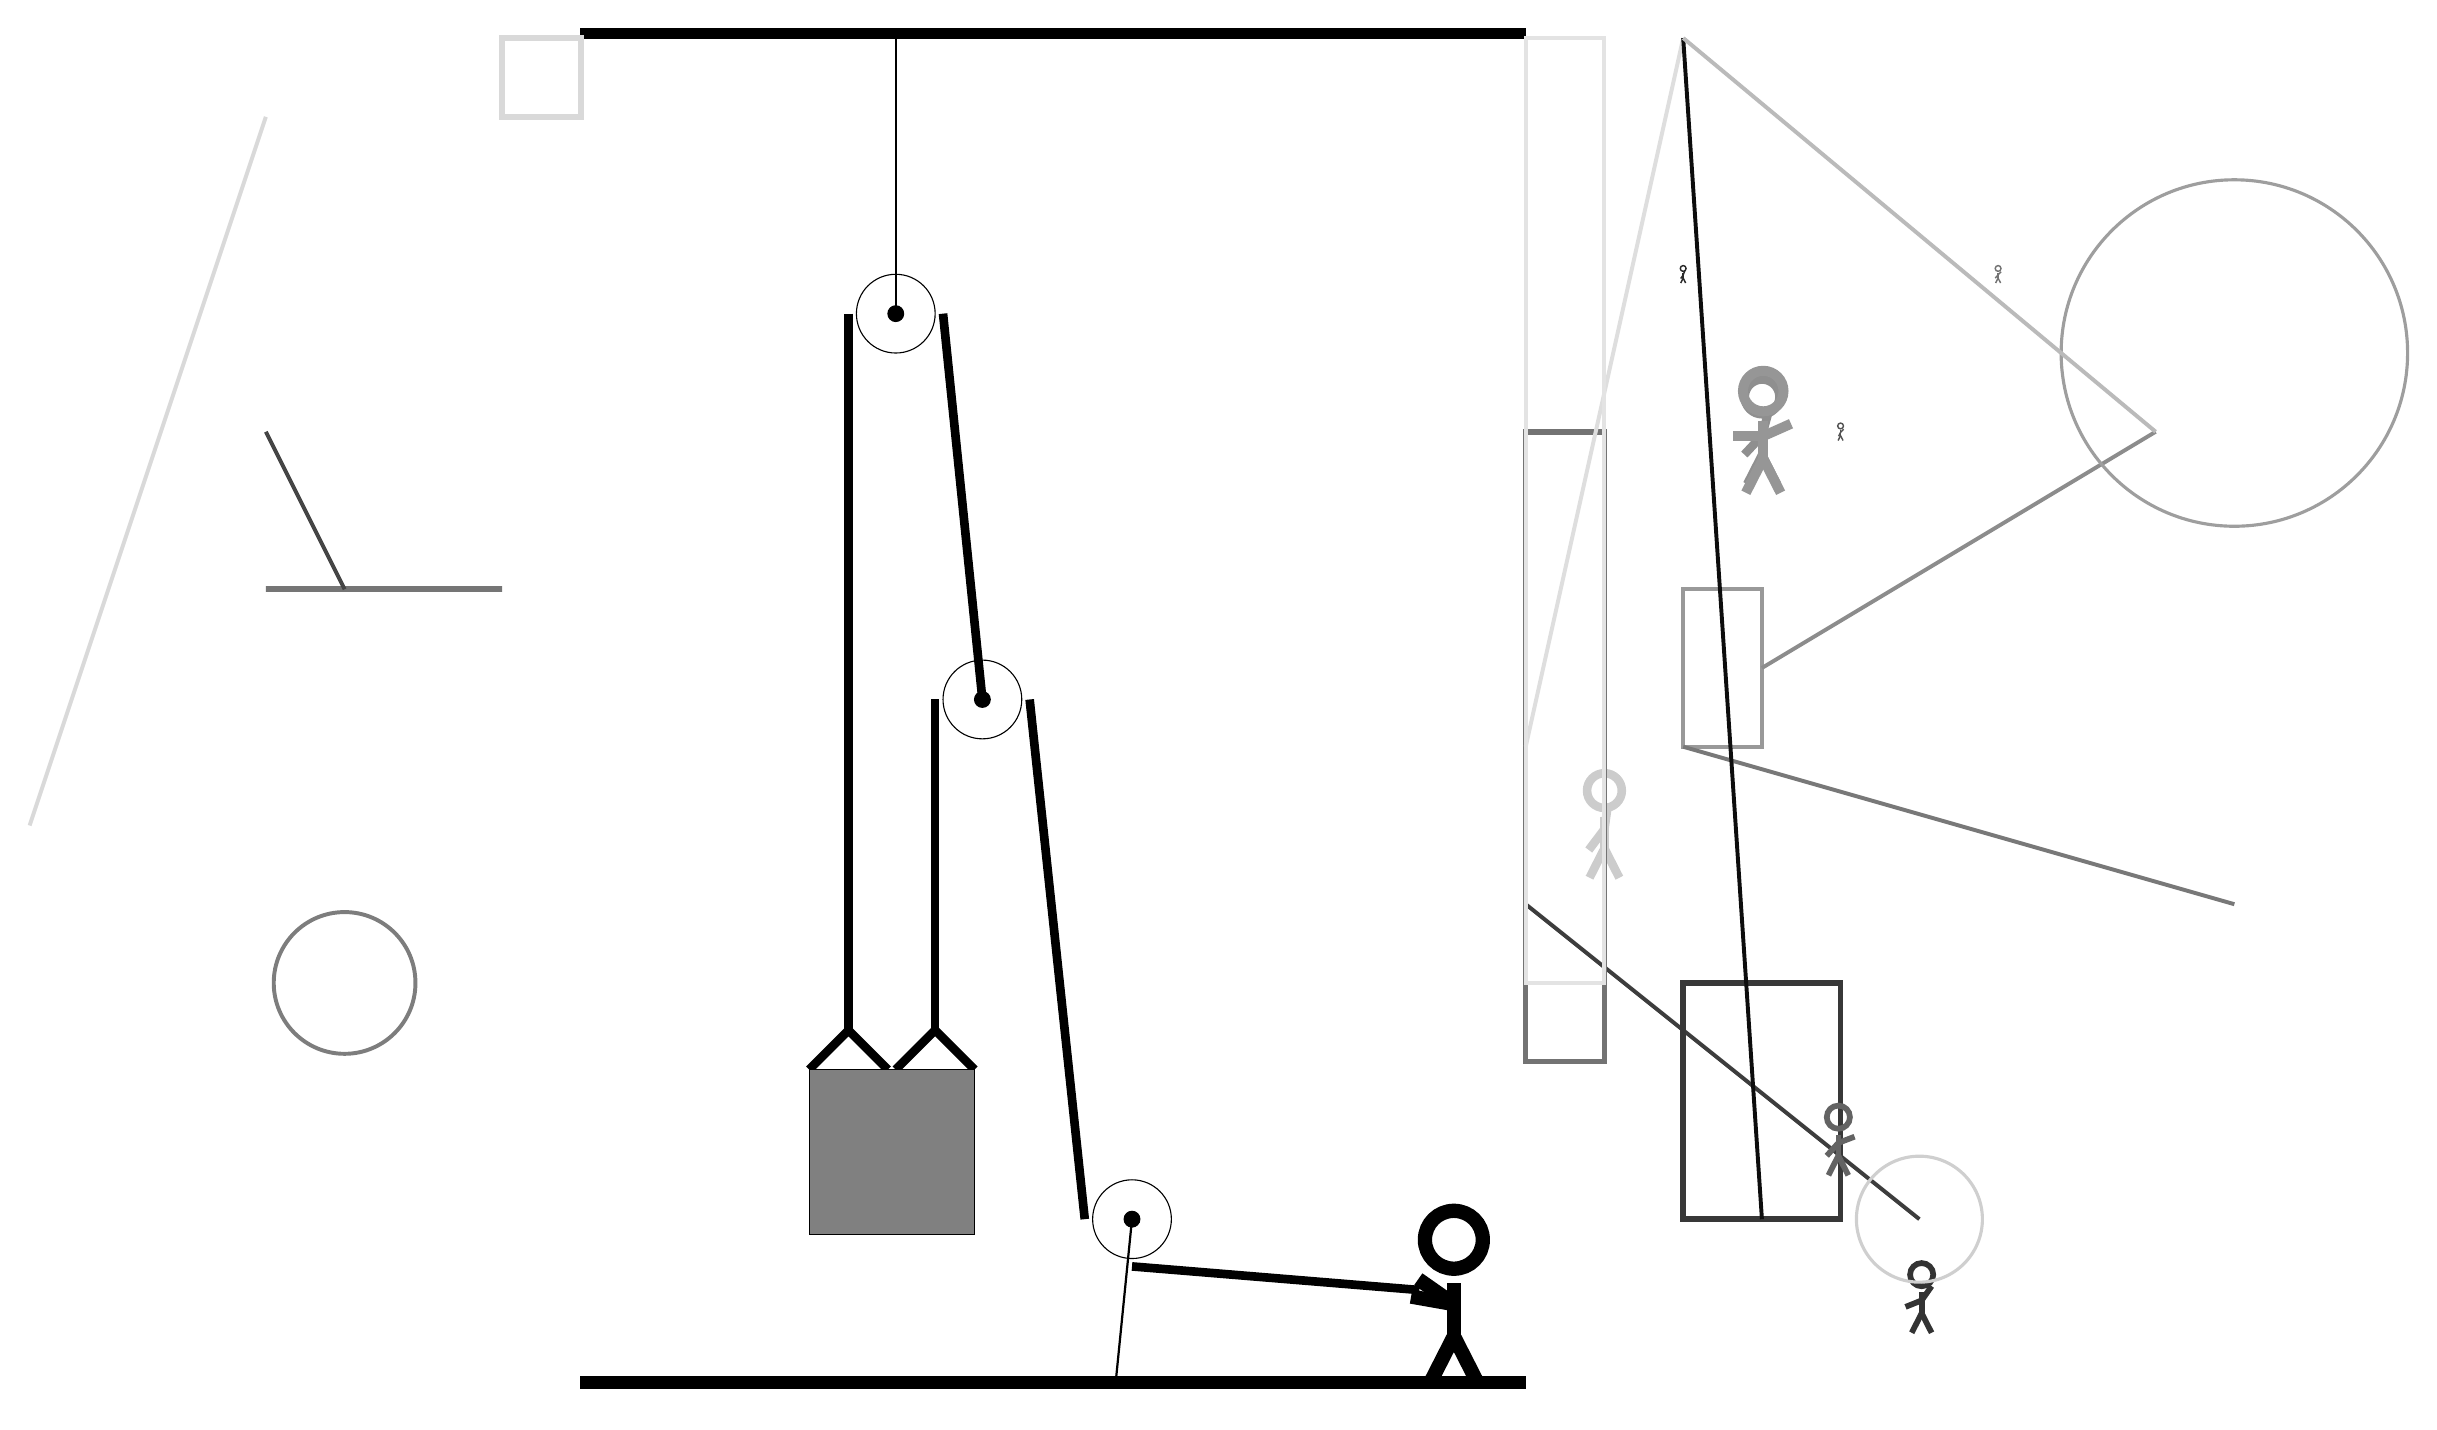
\begin{tikzpicture}
			%%%%% START %%%%%
			
			\draw[fill=black] (-2, 14) rectangle (10, 14.125);
			
			\draw (2, 10.5) circle (0.5);
			\draw[fill=black] (2, 10.5) circle (0.1);
			\draw[thick] (2, 10.5) -- (2, 14);
			
			\draw[line width=0.5mm, color=black!40] (12, 5) rectangle (13, 7);
			
			\draw[line width=0.5mm, color=black!45](13, 6) -- (18, 9);
			\draw[line width=0.7mm, color=black!54] (-3, 7) rectangle (-6, 7);
			\draw[line width=0.7mm, color=black!15] (-2, 14) rectangle (-3, 13);
			\draw[line width=0.5mm, color=black!76](10, 3) -- (15, -1);
			
			\node[line width=0.4mm, color=black!20] at (11, 4) {\Strichmaxerl[6][53][82]};
			
			\draw[line width=0.7mm, color=black!55] (10, 1) rectangle (11, 9);
			\node[line width=0.3mm, color=black!44] at (13, 9) {\Strichmaxerl[6][47][75]};
			\draw[line width=0.5mm, color=black!13](12, 14) -- (10, 5);
			\node[line width=0.7mm, color=black!80] at (15, -2) {\Strichmaxerl[4][22][55]};
			
			\draw[line width=0.5mm, color=black!73](-6, 9) -- (-5, 7);
			
			\draw[line width=0.7mm, color=black!78] (12, -1) rectangle (14, 2);
			\draw[line width=0.5mm, color=black!53](12, 5) -- (19, 3);
			
			\draw[line width=0.5mm, color=black!95](13, -1) -- (12, 14);
			\draw[line width=0.5mm, color=black!15](-6, 13) -- (-9, 4);
			\node[line width=0.3mm, color=black!84] at (12, 11) {\Strichmaxerl[1][56][68]};
			
			\node[line width=0.6mm, color=black!61] at (14, 0) {\Strichmaxerl[4][48][21]};
			\node[line width=0.6mm, color=black!55] at (16, 11) {\Strichmaxerl[1][48][47]};
			\node[line width=0.2mm, color=black!41] at (13, 9) {\Strichmaxerl[7][0][24]};
			\draw[line width=0.5mm, color=black!11] (11, 14) rectangle (10, 2);
			\draw [line width=0.4mm, color=black!38](19, 10) circle (2.2);
			\draw [line width=0.4mm, color=black!19](15, -1) circle (0.8);
			
			\draw [line width=0.5mm, color=black!51](-5, 2) circle (0.9);
			\draw[line width=0.5mm, color=black!27](12, 14) -- (18, 9);
			\node[line width=0.2mm, color=black!68] at (14, 9) {\Strichmaxerl[1][63][45]};
			
			\draw (3.1, 5.6) circle (0.5);
			\draw[fill=black] (3.1, 5.6) circle (0.1);
			
			\draw (5, -1) circle (0.5);
			\draw[fill=black] (5, -1) circle (0.1);
			\draw[thick] (5, -1) -- (4.8, -3);
			
			\draw[line width = 1.1mm]  (0.9, 0.9) -- (1.4, 1.4) -- (1.9, 0.9);
			\draw[line width = 1.1mm]  (2.0, 0.9) -- (2.5, 1.4) -- (3.0, 0.9);
			\draw[fill=black!50] (0.9, 0.9) rectangle (3.0, -1.2);
			
			\draw[line width = 1.1mm] (1.4, 10.5) -- (1.4, 1.4);
			\centerarc[line width = 1.1mm](2, 10.5)(0:180:0.6);
			\draw[line width = 1.1mm] (2.6, 10.5) -- (3.1, 5.6);
			\draw[line width = 1.1mm] (2.5, 5.6) -- (2.5, 1.4);
			\centerarc[line width = 1.1mm](3.1, 5.6)(0:180:0.6);
			\draw[line width = 1.1mm] (3.7, 5.6) -- (4.4, -1);
			\centerarc[line width = 1.1mm](5, -1)(180:270:0.6);
			\draw[line width = 1.1mm] (5, -1.6) -- (8.65, -1.9);
			
			\node at (9, -2) {\Strichmaxerl[10][-35][170]};
			
			\draw[fill=black] (-2, -3) rectangle (10, -3.15);
			
			%%%%% END %%%%%
		\end{tikzpicture}
	\end{figure}	
\end{document}